\subsubsubsection{Prijavljivanje korisnika}

\begin{itemize}
    \item Kratak opis:
        \begin{itemize}
            \item Korisnik koristi prethodno zapamćene informacije za prijavljivanje na aplikaciju.
        \end{itemize}
    \item Učesnici:
        \begin{itemize}
            \item Registrovani korisnik HelloFresh aplikacije.
        \end{itemize}
    \item Preduslovi:
        \begin{itemize}
            \item Korisnik mora da bude registrovan.
        \end{itemize}
    \item Postuslovi:
        \begin{itemize}
            \item Korisnik je uspešno pristupio svom nalogu.
        \end{itemize}
    \item Osnovni tok:
        \begin{enumerate}
            \item Korisnik pristupa veb stranici i otvara formu za prijavljivanje.
            \item Korisnik unosi svoje korisničko ime i lozinku koju je koristio pri registraciji.
            \item Sistem proverava postojanje i tačnost podataka i prosleđuje korisnika dalje ka osnovnom interfejsu aplikacije.
        \end{enumerate}
    \item Alternativni tok:
        \begin{itemize}
            \item[2.a] Ukoliko korisnik ne može da se seti svojih podataka dobija mejl sa informacijama o koracima za promenu lozinke. Nakon otvaranja mejla, slučaj upotrebe se nastavlja od koraka 2.
			\item[3.a] Ukoliko korisnik ne unese validne podatke sistem ga obaveštava o greški prilikom prijavljivanja. Slučaj upotrebe se nastavlja od koraka 2.
            \item[3.b] Ukoliko korisnik više puta ne uspe da se prijavi sa unetim podacima, dobija zabranu pokušaja na 1h. Nakon tog perioda, slučaj upotrebe se nastavlja od koraka 2.
        \end{itemize}
    \item Dodatne informacije:
        \begin{itemize}
            \item Zabrana prijavljivanja nakon nekoliko pokušaja obezbeđuje da server i korisnički podaci budu zaštićeni od 'brute force' napada.
        \end{itemize}
\end{itemize}

\begin{figure}[H]
\begin{center}
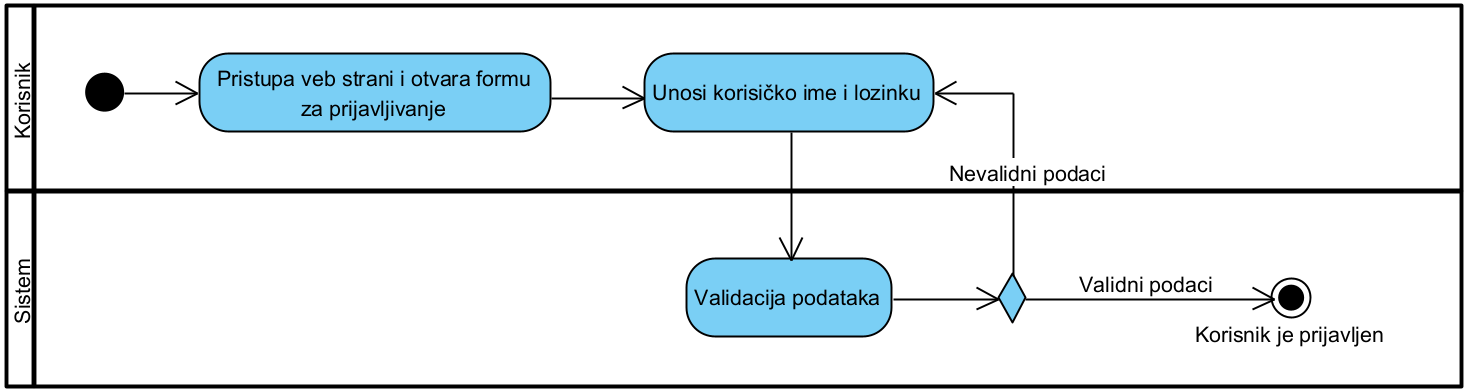
\includegraphics[width=\textwidth]{Pictures/activity_user_login.png}
\end{center}
    \caption{Dijagram aktivnosti prijavljivanja klijenta}
\label{fig:ActivityUserLogin}
\end{figure}
